%Preamble
\documentclass{article}
\usepackage{hyperref}
\usepackage[
    type={CC},
    modifier={by-nc-sa},
    version={3.0},
]{doclicense}
\usepackage[landscape]{geometry}
\usepackage{url}
\usepackage{multicol}
\usepackage{amsmath}
\usepackage{dsfont}
\usepackage{esint}
\usepackage{amsfonts}
\usepackage{tikz}
\usetikzlibrary{decorations.pathmorphing}
\usepackage{amsmath,amssymb}

\usepackage{colortbl}
\usepackage{xcolor}
\usepackage{mathtools}
\usepackage{amsmath,amssymb}
\usepackage{enumitem}
\makeatletter

\newcommand*\bigcdot{\mathpalette\bigcdot@{.5}}
\newcommand*\bigcdot@[2]{\mathbin{\vcenter{\hbox{\scalebox{#2}{$\m@th#1\bullet$}}}}}
\makeatother

\title{MECH 260 Formula Sheet}
\usepackage[english]{babel}
\usepackage[utf8]{inputenc}

\renewcommand{\baselinestretch}{1.15}

\advance\topmargin-.8in
\advance\textheight3in
\advance\textwidth3in
\advance\oddsidemargin-1.5in
\advance\evensidemargin-1.5in
\parindent0pt
\parskip2pt
\newcommand{\hr}{\centerline{\rule{3.5in}{1pt}}}
%\colorbox[HTML]{e4e4e4}{\makebox[\textwidth-2\fboxsep][l]{texto}

% Definitions for shortcuts
\newcommand{\ih}{\hat{i}}
\newcommand{\jh}{\hat{j}}
\newcommand{\kh}{\hat{k}}
\newcommand{\uh}{\hat{u}}
\newcommand{\vx}{\vec{x}}
\newcommand{\vy}{\vec{y}}
\newcommand{\vz}{\vec{z}}
\newcommand{\vr}{\vec{r}}
\newcommand{\vs}{\vec{s}}
\newcommand{\vv}{\vec{v}}
\newcommand{\va}{\vec{a}}
\newcommand{\vF}{\vec{F}}
\newcommand{\vE}{\vec{E}}
\newcommand{\f}{\mathrm{f}}
\newcommand{\Ra}{\Rightarrow}
\newcommand{\brangle}[1]{\left\langle #1 \right\rangle}
\newcommand{\brround}[1]{\left( #1 \right)}
\newcommand{\brcurly}[1]{\left\{ #1 \right\}}
\newcommand{\brsquare}[1]{\left[ #1 \right]}
\newcommand{\brvertical}[1]{\left| #1 \right|}
\newcommand{\matrixx}[1]{\left[\begingroup        \renewcommand{\arraystretch}{1}\begin{matrix} #1 \end{matrix}\endgroup\right]}
\newcommand{\eqnsystem}[1]{\left\{\begin{matrix} #1 \end{matrix}\right.}
\newcommand{\detmatrix}[1]{\left|\begin{matrix} #1
\end{matrix}\right|}
\newcommand{\R}{\mathds{R}}
\newcommand{\Z}{\mathds{Z}}
\newcommand{\N}{\mathds{N}}
\newcommand{\eval}[1]{\left. #1 \right|}
\newcommand{\augmatrix}[2]{\left[\begin{array}{#1|c}#2\end{array}\right]}
\newcommand{\lap}[1]{\Lap\brcurly{#1}}
\newcommand{\ilap}[1]{\Lap^{-1}\brcurly{#1}}
\newcommand{\para}{\parallel}
\newcommand{\formula}[2]{\begin{center} \begin{tcolorbox}[text width = #1] $$#2$$\end{tcolorbox}\end{center}}

%New operators
\DeclareMathOperator{\arccot}{arccot}
\DeclareMathOperator{\arccsc}{arccsc}
\DeclareMathOperator{\arcsec}{arcsec}
\DeclareMathOperator{\sgn}{sgn}


\begin{document}

\begin{center}{\huge{\textbf{MECH 260 - Unofficial Formula Sheet}}}\\
\end{center}
\begin{multicols*}{2}

\tikzstyle{mybox} = [draw=black, fill=white, very thick,
    rectangle, rounded corners, inner sep=10pt, inner ysep=10pt]
\tikzstyle{fancytitle} =[fill=black, text=white, font=\bfseries]

\renewcommand{\arraystretch}{1.7}

%------------ Stress and Strain ---------------
\begin{tikzpicture}
\node [mybox] (box){%
    \begin{minipage}{0.45\textwidth}
    \textbf{Normal Stress and Strain}
    \hrule
    \vspace{0.1cm}
    \small{
    \begin{tabular}{lp{8cm} l}
        Stress & $\sigma=\dfrac{F}{A_\perp}$\\
        Strain & $\varepsilon=\dfrac{\delta}{l_0}$\\
        Young's Modulus & $E=\dfrac{\sigma}{\varepsilon}$\\
        Deflection & $\delta=\dfrac{Fl}{AE}$\\
        Poisson's Ratio & $\varepsilon_{x,y}=\dfrac{-\nu}{E}\sigma_z$\\
        Normal Strain & $\varepsilon_{x|y|z}=\displaystyle{\frac{1}{E}}\brround{\sigma_{\para}-\nu(\sigma_{\perp1}+\sigma_{\perp2})}$\\
        Normal Stress & $\sigma_{x|y|z}=\displaystyle{\brround{\frac{E}{(1+\nu)(1-2\nu)}}\brround{(1-\nu)\varepsilon_\para+\nu(\varepsilon_{\perp1}+\varepsilon_{\perp2})}}$\\
        Matrix Form & $\matrixx{\varepsilon_x\\\varepsilon_y\\\varepsilon_z}=\dfrac{1}{E}\matrixx{1&-\nu&-\nu\\-\nu&1&-\nu\\-\nu&-\nu&1}\matrixx{\sigma_x\\\sigma_y\\\sigma_z}$
    \end{tabular}
    }\vspace{0.2cm}\\
    \normalsize
    \textbf{Volumetric Stress and Strain}
    \hrule
    \small{
    \begin{tabular}{lp{8cm} l}
        Volumetirc Strain & $\varepsilon_V=\dfrac{\Delta V}{V_0}\approx \varepsilon_x+\varepsilon_y+\varepsilon_z=\brround{\dfrac{1-2\nu}{E}}(\sigma_x+\sigma_y+\sigma_z)$\\
        Bulk Modulus & $K=\dfrac{E}{3(1-2\nu)}$
    \end{tabular}
    }\vspace{0.2cm}\\
    \normalsize
    \textbf{Shear Stress and Strain}
    \hrule
    \small{
    \begin{tabular}{lp{8cm}}
    Shear Stress & $\tau=\dfrac{V}{A_\para}$\\
    Shear Strain & $\gamma=\dfrac{\delta}{l}$\\
    Shear Modulus & $G=\dfrac{\tau}{\gamma}$\\
    Matrix Form & $\matrixx{\tau_{xy}\\\tau_{xz}\\\tau_{yz}}=\matrixx{G&0&0\\0&G&0\\0&0&G}\matrixx{\gamma_{xy}\\\gamma_{xz}\\\gamma_{yz}}$
    \end{tabular}
    }\vspace{0.2cm}\\
    \normalsize
    \textbf{Thermal Stress and Strain}
    \hrule
    \small{
    \begin{tabular}{lp{8cm}}
    Thermal Strain & $\varepsilon=\alpha_L\Delta T$\\
    & $\varepsilon_V=\alpha_V\Delta T\approx 3\alpha_L\Delta T$\\
    Total Strain & $\varepsilon_{x|y|z}=\varepsilon_{\text{normal}}+\alpha_L\Delta T$\\
    Total Stress & $\sigma_{x|y|z}=\displaystyle{\sigma_{\text{normal}}-\brround{\frac{E}{1-2\nu}}\alpha_L\Delta T}$\\
    Volumetric & $\varepsilon_V=\brround{\dfrac{1-2\nu}{E}}(\sigma_x+\sigma_y+\sigma_z)+3\alpha_L\Delta T$\\
     & $\sigma_x+\sigma_y+\sigma_z=\brround{\dfrac{E}{1-2\nu}}\brround{\varepsilon_V-3\alpha_L\Delta T}$
    \end{tabular}
    }
    \end{minipage}
};
%------------ Stress and Strain ---------------------
\node[fancytitle, right=10pt] at (box.north west) {Average Stress and Strain};
\end{tikzpicture}

%------------ Stress and Strain ---------------
\begin{tikzpicture}
\node [mybox] (box){%
    \begin{minipage}{0.45\textwidth}
    \textbf{Nonuniform Stress}
    \hrule
    \vspace{0.1cm}
    \small{
    \begin{tabular}{lp{8cm} l}
        Safety Factor & $f_s=\eqnsystem{\dfrac{\sigma_{Y}}{|\sigma_{\text{nom}}|} & \text{(ductile)}\\
        \dfrac{\sigma_{UT}}{|\sigma_{\text{max}}|} & \text{(brittle, tension)}\\
        \dfrac{|\sigma_{UC}|}{|\sigma_{\text{max}}|} & \text{(brittle, compression)}}$\\
        Nominal Stress & $\sigma_{\text{nominal}}=\dfrac{F_{\text{avg}}}{A_{\text{min}}}$\\
        K Value & $K=\dfrac{\sigma_{\text{max}}}{\sigma_{\text{nominal}}}$
    \end{tabular}
    }
    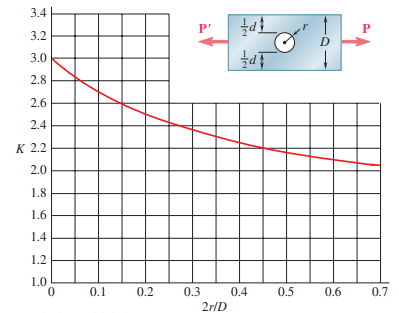
\includegraphics[scale=0.9]{graph1.png}\\
    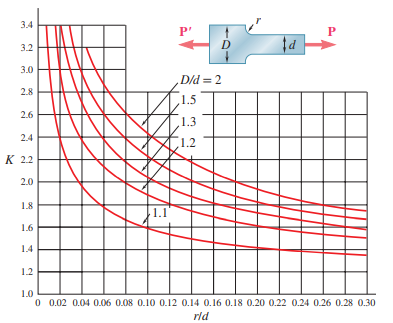
\includegraphics[scale=1]{graph2.png}
    \end{minipage}
};
%------------ Stress and Strain ---------------------
\node[fancytitle, right=10pt] at (box.north west) {Nonuniform Stress and Strain};
\end{tikzpicture}

%------------ Torsion ---------------
\begin{tikzpicture}
\node [mybox] (box){%
    \begin{minipage}{0.45\textwidth}
    \textbf{Torsion}
    \hrule
    \vspace{0.1cm}
    \small{
    \begin{tabular}{lp{8cm} l}
        Shear Strain & $\gamma(r)=\dfrac{r}{l}\phi$\\
        Shear Stress & $\dfrac{\tau(r)}{r}=\dfrac{T}{J}=\dfrac{G}{l}\phi$\\
        Polar Moment of Area & $J=\eqnsystem{\frac{\pi}{2}r_{\text{surf}}^4 & \text{(Solid Circular Shaft)}\\
        \frac{\pi}{2}(r_{\text{surf}}^4-r_{\text{in}}^4) & \text{(Hollow Circular Shaft)}\\
        2\pi tr_{\text{surf}}^3 & \text{(Hollow Circular, $t\ll r_{\text{surf}}$)}}$\\
        & $J_{\text{rectangle}} = \dfrac{bh(b^2+h^2)}{12}$\\
    \end{tabular}
    }
    \normalsize
    \textbf{Bending}
    \hrule
    \vspace{0.1cm}
    \small{
    \begin{tabular}{lp{8cm} l}
        Bending & $\dfrac{\sigma_x}{-y}=\dfrac{M}{I_z}=\dfrac{E}{\rho}\quad \text{(where $\rho$ is radius of curvature)}$\\
        Center of Area & $y_C^*=\dfrac{1}{A_{\text{total}}}\sum y_i^*A_i$\\
        Parallel Axis Theorem & $(I_z)_{O}=(I_z)_C+A\Delta y^2$\\
        Rectangular Moment of Area & $(I_z)_{\text{rectangle}}=\dfrac{bh^3}{12}$\\
         & $(I_z)_{\text{circle}}=\dfrac{J}{2}$\\
         Summation of $I_z$ & $I_z = \sum I_{z,i} + \sum A_i(y^*_{NA}-y^*_{NA,i})^2$\\
         Moment of Area & $J=I_z+I_y$\\
         Composite Cross Sections & $b_{\text{transformed}}=b\brround{\frac{E}{E_{\text{ref}}}}$\\
         & $\displaystyle{\frac{\sigma_x}{-y}\brround{\frac{E_{\text{ref}}}{E}}=\frac{M}{I_z}=\frac{E_{\text{ref}}}{\rho}}$
    \end{tabular}
    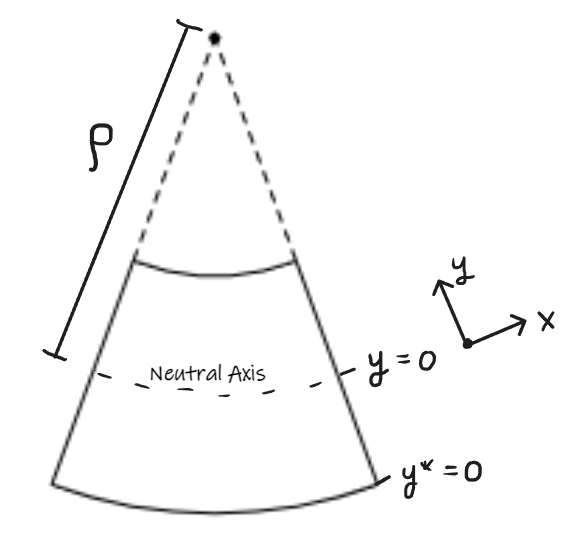
\includegraphics[scale=0.5]{BendingCrossSection.png}\\ $y=y^*-y_{NA}^*$
    }
    \end{minipage}
};
%------------ Torsion ---------------------
\node[fancytitle, right=10pt] at (box.north west) {Torsion and Bending};
\end{tikzpicture}

%------------ Mohr Circle ---------------
\begin{tikzpicture}
\node [mybox] (box){%
    \begin{minipage}{0.45\textwidth}
    \textbf{Stress Transformation}
    \hrule
    \vspace{0.1cm}
    \small
    \begin{tabular}{lp{8cm} l}
        $\sigma_{x'}=\brround{\frac{\sigma_x+\sigma_y}{2}}+\brround{\frac{\sigma_x-\sigma_y}{2}}\cos2\theta+\tau_{xy}\sin2\theta$\\
        $\sigma_{y'}=\brround{\frac{\sigma_x+\sigma_y}{2}}-\brround{\frac{\sigma_x-\sigma_y}{2}}\cos2\theta-\tau_{xy}\sin2\theta$\\
        $\tau_{x'y'}=-\brround{\frac{\sigma_x-\sigma_y}{2}}\sin2\theta+\tau_{xy}\cos2\theta$
    \end{tabular}\\
    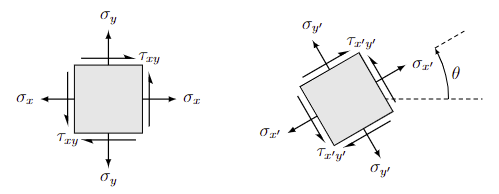
\includegraphics[scale=1]{TransformationCube.png}\\
    Note that $\theta$ for the stress cube corresponds to $2\theta$ in Mohr Circle space.\\
    \normalsize
    \textbf{Principal Planes and Max Shear Stress}
    \hrule
    \vspace{0.1cm}
    \small{
    \begin{tabular}{lp{8cm} l}
        Center Point & $C = \sigma_{avg} = \frac{\sigma_x + \sigma_y}{2}$\\
        Radius & $R = \sqrt{\left(\frac{\sigma_x - \sigma_y}{2}\right)^2 + \left(\tau_{xy}\right)^2}$\\
        Principal Stresses & $\sigma_{p1,p2} = C\pm R$\\
        Principal Angles & $2\theta_{p1} = \tan^{-1}\left(\frac{2\tau_{xy}}{\sigma_x-\sigma_y}\right)$\\
            & $\theta_{p2} = \theta_{p1} + 90^{\circ}$\\
        Max Shear Stress & $\tau_{max} = R$\\
        Critical Planes & $\theta_{cp1,cp2} = \theta_{p1,p2} + 45^{\circ}$\\
    \end{tabular}
    }
    \normalsize
    \textbf{Failure Criteria}
    \hrule
    \vspace{0.1cm}
    \small
    \begin{tabular}{lp{9cm} l}
        Tresca & $\sigma_{\text{max}}-\sigma_{\text{min}}=2\tau_{\text{max}}=\dfrac{\sigma_Y}{f_s^{\text{Tresca}}}$\\
        von Mises & $\frac{1}{2}\brround{(\sigma_1-\sigma_2)^2+(\sigma_2-\sigma_3)^2+(\sigma_1-\sigma_3)^2}=\brround{\dfrac{\sigma_Y}{f_s^{\text{vM}}}}^2$\\
        Mohr & $\displaystyle{\frac{\sigma_{\text{max}}}{\sigma_{UT}}-\frac{\sigma_{\text{min}}}{|\sigma_{UC}|}=\frac{1}{f_s^{\text{Mohr}}}}$ (for brittle materials)
    \end{tabular}\\
    \normalsize
    \textbf{Thin-Walled Pressure Vessels}
    \hrule
    \vspace{0.1cm}
    \small
    \begin{tabular}{lp{3cm} l}
        Sphere & $\sigma_\theta^{\text{sph}}=\dfrac{Pr}{2t}$\\
        Cylinder & $\sigma_{\text{ax}}=\dfrac{Pr}{2t}$
        & $\sigma_\theta^{\text{cyl}}=\dfrac{Pr}{t}$
    \end{tabular}
    \end{minipage}
};
%------------ Mohr Circle ---------------------
\node[fancytitle, right=10pt] at (box.north west) {Mohr's Circle};
\end{tikzpicture}



%-------------------Authorship-----------------------
\begin{center}
    \framebox{
    \parbox[t][.5cm]{10.5cm}{
    \addvspace{0.2cm} \centering 
    \footnotesize Compiled by Tyler Wilson, Julian Lapenna, and Spencer Bradbury 2022 
    } 
}
\end{center}
\end{multicols*}



\end{document}
